\documentclass[tikz]{standalone}

\usepackage{ctex}

\usepackage{tikz}

\tikzset{>=latex}

\usetikzlibrary{decorations.markings}
\tikzset{->-/.style={decoration={
  markings,
  mark=at position .5 with {\arrow{>}}},postaction={decorate}}}
\tikzset{-<-/.style={decoration={
  markings,
  mark=at position .5 with {\arrow{<}}},postaction={decorate}}}


\newcommand{\xOy}[4]{
	\draw[thick, <->](0, #4)node[left]{$#3$}--(0, 0)node[shift={(-135:7pt)}]{$O$}--(#2, 0)node[right]{$#1$}
}

\usepackage{BOONDOX-cal}

\newcommand*{\phs}{\mathcal s}
\newcommand*{\phl}{\mathcal l}
\newcommand*{\phg}{\mathcal g}
\newcommand*{\phaq}{\mathcal{a\!q}\!}
\newcommand*{\phel}{\mathcal{el}\!}
\newcommand*{\crt}{\mathrm C}
% \newcommand*{\hji}{\scalebox{.4}[1]{火}\hspace{-4.3pt}\scalebox{.4}[1]{火}\hspace{-1pt}\scalebox{.7}[1]{积}}

\definecolor{gr1}{gray}{.9}
\definecolor{gr2}{gray}{.8}
\definecolor{gr3}{gray}{.7}
\definecolor{gr4}{gray}{.6}
\definecolor{grmixed}{gray}{.75833}%1-29/120

\definecolor{clg}{gray}{.95}
\definecolor{cll}{gray}{.8}
\definecolor{cls}{gray}{.6}
\definecolor{clgl}{gray}{.875}
\definecolor{clls}{gray}{.7}
\definecolor{clsg}{gray}{.775}


\usetikzlibrary{patterns}

\begin{document}

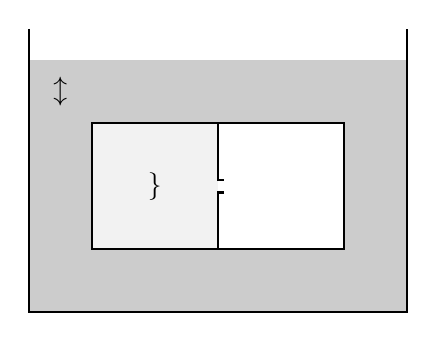
\begin{tikzpicture}[thick, scale=0.8]
    % \fill[white](-1, 5)rectangle(7, -1);
    \fill[cll](0, 0)rectangle(6, 4);
    \draw(0, 4.5)--(0, 0)--(6, 0)--(6, 4.5);
    \node at (.5, 3.5) {$\phl$};
    \fill[clg](1, 1)rectangle(3, 3);
    \node at (2, 2) {$\phg$};
    \fill[white](3, 1)rectangle(5, 3);
    \draw(1, 1)rectangle(5, 3);
    \draw(3, 1)--(3, 1.9)--(3.1, 1.9);
    \draw(3, 3)--(3, 2.1)--(3.1, 2.1);
    % \draw[->](3, 3.3)--(3, 4.3);
\end{tikzpicture}

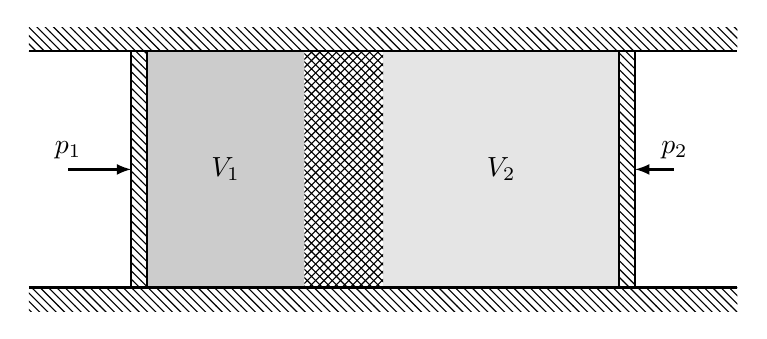
\begin{tikzpicture}[thick]
    % \fill[white](-1, -1)rectangle(9, 4);
    \fill[gr2](1.5, 0)rectangle(3.5, 3);
    \fill[gr1](4.5, 0)rectangle(7.5, 3);
    \draw(0, 0)--(9, 0);
    \draw(0, 3)--(9, 3);
    \fill[pattern=north west lines](0, 0)rectangle(9, -.3);
    \fill[pattern=north west lines](0, 3)rectangle(9, 3.3);
    \draw[pattern=north west lines](1.5-.2, 0)rectangle(1.5, 3);
    \draw[<-](1.5-.2, 1.5)--(.5, 1.5)node[above]{$p_1$};
    \node at(2.5, 1.5){$V_1$};
    \draw[pattern=north west lines](7.5, 0)rectangle(7.5+.2, 3);
    \draw[<-](7.5+.2, 1.5)--(8.2, 1.5)node[above]{$p_2$};
    \node at(6, 1.5){$V_2$};
    \fill[pattern=crosshatch](3.5, 0)rectangle(4.5, 3);
\end{tikzpicture}

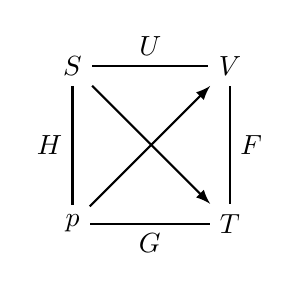
\begin{tikzpicture}[thick]
    \node(s)at(0, 2){$S$};
    \node(v)at(2, 2){$V$};
    \node(p)at(0, 0){$p$};
    \node(t)at(2, 0){$T$};
    \draw(s)--(v)node[midway, above]{$U$};
    \draw(s)--(p)node[midway, left]{$H$};
    \draw(t)--(v)node[midway, right]{$F$};
    \draw(t)--(p)node[midway, below]{$G$};
    \draw[->](s)--(t);
    \draw[->](p)--(v);
\end{tikzpicture}

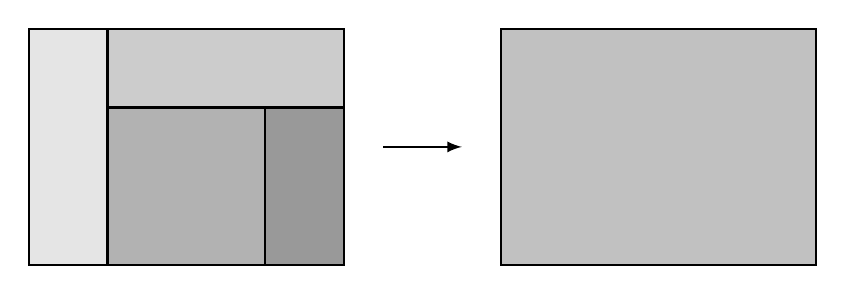
\begin{tikzpicture}[thick]
    \draw[fill=gr1](0, 0)rectangle(1, 3);
    \draw[fill=gr2](1, 2)rectangle(4, 3);
    \draw[fill=gr3](1, 0)rectangle(3, 2);
    \draw[fill=gr4](3, 0)rectangle(4, 2);
    \draw[->](4.5, 1.5)--(5.5, 1.5);
    \begin{scope}[xshift=6cm]
        \draw[fill=grmixed](0, 0)rectangle(4, 3);
    \end{scope}
\end{tikzpicture}

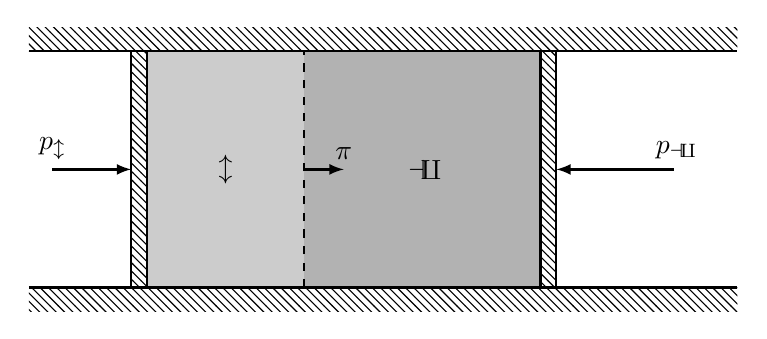
\begin{tikzpicture}
    \fill[cll](1.5, 0)rectangle(3.5, 3);
    \fill[clls](3.5, 0)rectangle(6.5, 3);
    \draw[thick](0, 0)--(9, 0);
    \draw[thick](0, 3)--(9, 3);
    \fill[pattern=north west lines](0, 0)rectangle(9, -.3);
    \fill[pattern=north west lines](0, 3)rectangle(9, 3.3);
    \draw[thick, pattern=north west lines](1.5-.2, 0)rectangle(1.5, 3);
    \draw[thick, <-](1.5-.2, 1.5)--(.5-.2, 1.5)node[above]{$p_\phl$};
    \node at(2.5, 1.5){$\phl$};
    \draw[thick, pattern=north west lines](6.5, 0)rectangle(6.5+.2, 3);
    \draw[thick, <-](6.5+.2, 1.5)--(8.2, 1.5)node[above]{$p_\phaq$};
    \node at(5, 1.5){$\phaq$};
    \draw[thick, dashed](3.5, 0)--(3.5, 3);
    \draw[thick, ->](3.5, 1.5)--(4, 1.5)node[above]{$\pi$};
\end{tikzpicture}

\usetikzlibrary{arrows.meta}
\begin{tikzpicture}[>=Stealth, thick, scale=3]
    \node(s)at(-1.732, 0){固$\phs$};
    \node(l)at(0, 1){液$\phl$};
    \node(g)at(0, -1){气$\phg$};
    \draw[arrows={->[left]}](s.-25)--(g.145)node[above, midway, sloped]{升华(sublimation)};
    \draw[arrows={->[left]}](g.155)--(s.-35)node[below, midway, sloped]{凝华(deposition)};
    \draw[arrows={->[left]}](s.35)--(l.-155)node[above, midway, sloped]{熔化(melting)};
    \draw[arrows={->[left]}](l.-145)--(s.25)node[below, midway, sloped]{凝固(freezing)};
    \draw[arrows={->[left]}](g.95)--(l.-95)node[above, midway, sloped]{液化(condensation)};
    \draw[arrows={->[left]}](l.-80)--(g.80)node[below, midway, sloped, rotate=180]{气化(vaporization)};
\end{tikzpicture}

\end{document}